\documentclass[12pt]{article}
\usepackage[margin=1in]{geometry}
\usepackage[utf8]{inputenc}
\usepackage[spanish]{babel}
\usepackage{parskip}
\usepackage{setspace}
\usepackage{amsmath, amssymb}
\usepackage{tikz}
\usepackage{hyperref} % Siempre debe ir al final.

% Opciones de Paquetes.
\decimalpoint           % {babel}
\onehalfspacing         % {setspace}
\graphicspath{{./img/}} % {graphics}

% Encabezado.
\title{Clase 1: Introducción a la Probabilidad y Métodos de Conteo.}
\author{Harvard Statistics 110: Probability.}
\date{}


\begin{document}

\maketitle

\begin{abstract}
\noindent El concepto de probabilidad ha ido cambiando desde que comenzó a formalizarse, pero su idea central se ha mantenido casi intacta, es por ello que en esta primera clase estudiaremos su primera definición (en ocasiones etiquetada como ``ingenua'' o como ``clásica''). También revisaremos algunos métodos de conteo que facilitan su cálculo.
\end{abstract}


\section{Introducción a la probabilidad.}

Muchas veces nos gustaría conocer de antemano el resultado de una acción que queremos realizar. Como no podemos saberlo de forma exacta, definimos ciertos escenarios y establecemos qué tan posible es que cada uno ocurra. El área de la matemática que describe numéricamente esa (in)certidumbre se conoce como \textbf{Probabilidad}.

Las primeras descripciones matemáticas de las probabilidades tienen su origen en los juegos de azar. Aquello se puede ver, por ejemplo, en la correspondencia realizada entre Pierre de Fermat y Blaise Pascal alrededor del año 1654.

No obstante, lo que se conoce como la ``definición ingenua (o clásica) de la probabilidad'' es adjudicada a Gerolamo Cardano un siglo antes de Fermat y Pascal. Para entenderla, debemos tener un conocimiento básico sobre teoría de conjuntos que veremos a continuación.

\subsection{Conceptos básicos de la teoría de conjuntos.}

\subsubsection{Conjuntos.}

Un \textbf{conjunto} es una colección abstracta y \textbf{no ordenada} de distintos objetos llamados \textbf{elementos} o miembros.

Una manera común de expresar un conjunto es usando el \textbf{método de Roster}, que consiste en enlistar todos sus elementos adentro de unos $\{ \ \}$. Por ejemplo, es posible escribir a los miembros $1$, $2$ y $7$ de un conjunto $A$ como:
\[
  A = \{1, \ 2, \ 7\}
\]
Otra forma de denotar a un conjunto es indicando la propiedad que cumplen sus elementos. Dicho método se conoce como \textbf{constructor de conjunto} (\textit{set builder})\footnote{Herbert Enderton en \textit{Elements of Set Theory} lo llama \textbf{método de abstracción} (1977: 4).}. A continuación tenemos un conjunto $V$ de enteros positivos menores a $15$.
\[
  V = \{x \in \mathbb{Z}^{+} \ | \ x < 15 \}
\]
El símbolo $\in$ indica la pertenencia de un objeto a un conjunto y su opuesto es denotado como $\notin$. Por otra parte, $|$ se lee de forma literal como ``tal que''.

El \textbf{conjunto que no tiene elementos} se conoce como \textbf{conjunto vacío} (o nulo) y se expresa como $\emptyset$, mientras que el que tiene \textbf{solo uno} (por ejemplo, $\{a\}$) se llama \textbf{singleton}.

\subsubsection{Subconjuntos y complemento de un conjunto.}

Un conjunto $B$ es un \textbf{subconjunto} de $A$ ($B \subseteq A$) \textbf{si todos sus elementos también son parte de $A$}. Si se cumple que $B \subseteq A$ y $A \subseteq B$, entonces $A = B$. En cambio, si $B \subseteq A$ y $A \nsubseteq B$, entonces $B$ es un \textbf{subconjunto propio} de $A$ ($A \subset B$).

Dos consecuencias de lo señalado sobre los subconjuntos son que $A \subseteq A$ (i.e, todo conjunto es un subconjunto de sí mismo) y que $\emptyset \subset A$ para todo $A$.\footnote{Es una \textbf{verdad vacua} (\textit{vacuous truth}): Esta afirmación sería falsa solo si $x \in \emptyset$ para $x \notin A$, pero eso es imposible ya que $\emptyset$ no tiene elementos. Por lo tanto, al no ser falsa, solo puede ser verdadera para todo $A$. Este razonamiento es usado por Paul Halmos en \textit{Naive Set Theory} (1974: 8).}

El \textbf{complemento} de $A$, $A^{c}$, es el conjunto de elementos que \textbf{no son parte de} $A$.
\[
  A^{c} = \{x \ | \ x \notin A\}
\]

\subsubsection{Operaciones sobre conjuntos.}

Sean $A$ y $B$ dos conjuntos. El conjunto que contiene a todos los \textbf{elementos de $A$ o $B$ o ambos} recibe el nombre de \textbf{unión} de $A$ y $B$ y es denotado como $A \cup B$.
\[
  A \cup B = \{x \ | \ x \in A \text{ o } x \in B\}
\]
La \textbf{intersección} de $A$ y $B$, $A \cap B$, corresponde al conjunto de todos los elementos que pertenecen \textbf{tanto a $A$ como a $B$}.
\[
  A \cap B = \{x \ | \ x \in A \text{ y } x \in B\}
\]
Si no hay elementos en común entre $A$ y $B$ o, en otras palabras, si $A \cap B = \emptyset$, se concluye que son \textbf{conjuntos disjuntos}.

Es posible considerar la unión o intersección de una \textbf{cantidad infinita de conjuntos}.

La \textbf{unión} de $\{A_{n}\}_{n = 1}^{\infty}$ es el conjunto del cual son parte todos los elementos que son \textbf{miembros de al menos un} $A_{n}$.
\[
  \bigcup_{n = 1}^{\infty} A_{n} = A_{1} \cup A_{2} \cup \ldots = \{x \ | \ x \in A_{n} \text{ para algún } n \}
\]
Mientras que la \textbf{intersección} de $\{A_{n}\}_{n = 1}^{\infty}$ es el conjunto que contiene a los elementos que son \textbf{miembros de todos} los $A_{n}$.
\[
  \bigcap_{n = 1}^{\infty} A_{n} = A_{1} \cap A_{2} \cap \ldots = \{x \ | \ x \in A_{n} \text{ para todo } n \}
\]
Un conjunto $M$ es una \textbf{Partición} de otro conjunto $A$ si consiste de una colección $A_{k} \subseteq M$, para $k = 1, \ 2, \ \ldots, \ n$, donde:

\begin{enumerate}
\item $\displaystyle \bigcup_{k = 1}^{n} A_{k} = M$.
\item $A_{i} \cap A_{j} = \emptyset$, para todo $i \neq j$.
\end{enumerate}

De las operaciones entre conjuntos se extraen las siguientes propiedades o leyes.

\begin{table}[hbt!]
\centering
\renewcommand{\arraystretch}{1.4}

\begin{tabular}{c c c}
\hline
Propiedad/Ley & Unión & Intersección \\
\hline
Conmutativa & $A \cup B = B \cup A$ & $A \cap B = B \cap A$ \\
Asociativa & $A \cup (B \cup C) = (A \cup B) \cup C$ & $A \cap (B \cap C) = (A \cap B) \cap C$ \\
Distributiva & $A \cap (B \cup C) = (A \cap B) \cup (A \cap C)$ & $A \cup (B \cap C) = (A \cup B) \cap (A \cup C)$ \\
de Morgan & $(A \cup B)^{c} = A^{c} \cap B^{c}$ & $(A \cap B)^{c} = A^{c} \cup B^{c}$ \\
\hline
\end{tabular}

\end{table}

\subsubsection{Cardinalidad de un conjunto.}

La \textbf{cardinalidad} o tamaño de un conjunto $A$, $|A|$, es un valor que indica la \textbf{cantidad de elementos} que pertenecen a $A$.

Solo es posible obtener la cardinalidad de un conjunto \textbf{finito}. Para aquellos que son \textbf{infinitos} existen dos tipos:

\begin{enumerate}
\item \textbf{Infinitos contables}: Si su tamaño es igual a la del conjunto de los \textbf{enteros positivos}.

\item \textbf{Infinitos incontables}.
\end{enumerate}

Si dos conjuntos $A$ y $B$ son \textbf{finitos}, es posible calcular la cardinalidad de su \textbf{unión} como:
\[
  |A \cup B| = |A| + |B| - |A \cap B|
\]

\subsubsection{Pares no ordenados y ordenados.}

Un \textbf{par no ordenado} (\textit{unordered pair}) $\{a, \ b\}$ es aquel conjunto que consiste exactamente de dos elementos distintos , $a$ y $b$, \textbf{no ordenados}. Esta última característica quiere decir que:
\[
  \{a, \ b\} = \{b, \ a\}
\]
Un \textbf{par ordenado} (\textit{ordered pair}) $(a, \ b)$ es una lista \textbf{ordenada} de solo dos elementos distintos $a$ y $b$. Estos últimos se indican por su posición: $a$ es la primera coordenada y $b$ la segunda de $(a, \ b)$. Por otra parte, se lo categoriza como ``\textbf{ordenado}'' si se cumple la siguiente condición:
\[
  (a, \ b) = (b, \ a) \iff a = b \text{ y } b = a
\]

\subsubsection{Multiconjuntos, tuplas y sucesiones.}

Los \textbf{multiconjuntos} son una colección \textbf{no ordenada finita o infinita} de objetos que \textbf{pueden repetirse}.

Las \textbf{tuplas} corresponden a \textbf{listas finitas ordenadas} de objetos distintos o \textbf{repetidos}. Se las menciona como ``\textbf{\textit{n}-tupla}'' si consisten de $n$ elementos.

En cuanto a las \textbf{sucesiones} (o secuencias), son una colección \textbf{ordenada finita o infinita de objetos} que pueden tener \textbf{elementos repetidos}.

\subsubsection{Producto cartesiano.}

El \textbf{producto cartesiano} entre dos conjuntos $A$ y $B$, $A \times B$, es el conjunto de \textbf{todos los pares ordenados} que pueden formarse entre \textbf{los elementos de ambos}.
\[
  A \times B = \{(a, \ b) \ | \ a \in A \text{ y } b \in B\}
\]

\subsection{Experimento, espacio muestral y evento.}

En probabilidades, un \textbf{experimento} suele ser entendido como cualquier proceso (real o hipotético) que produce \textbf{uno de varios} resultados posibles y que puede ser repetido en una cantidad infinita de veces.

El \textbf{espacio muestral} es el conjunto de todos los resultados posibles de un experimento. Este puede ser finito, infinito contable o incontable.

Bertsekas y Tsitsiklis detallan en \textit{Introduction to Probability} que al construir un espacio muestral debemos tener en consideración lo siguiente (2008: 7):

\begin{itemize}
\item Sus elementos deben ser \textbf{mutuamente excluyentes}: Al finalizar un experimento, debe ocurrir solo uno de todos sus elementos.\footnote{Por ejemplo, el espacio muestral del lanzamiento único de un dado es $\{1, \ 2, \ 3, \ 4, \ 5, \ 6\}$. Este punto indica que cuando deja de rodar luego de tirarlo, debemos obtener solo uno de sus seis elementos.}

\item Debe ser \textbf{colectivamente exhaustivo}: En él se encuentran todos los resultados posibles tal que el único que se obtiene al finalizar el experimento siempre será miembro de este conjunto, independiente de lo que haya ocurrido en ese proceso.

\item Los resultados posibles deben ser solo los del interés del experimentador/a. Cualquier información irrelevante debe ser desechada de este conjunto.
\end{itemize}

Un \textbf{evento} (o suceso) se define como un subconjunto bien definido del espacio muestral.

\subsection{Definición ``ingenua'' de probabilidad.}

Sean $S$ el espacio muestral de un experimento, $A \subseteq S$ un evento de éste y $P$ una función real. La \textbf{definición ingenua} de las probabilidades indica que si se cumple que:

\begin{enumerate}
\item El espacio muestral ($S$) es \textbf{finito}.
\item Cada resultado es \textbf{igualmente probable}\footnote{Es decir, todos tienen la misma posibilidad de ocurrir.}.
\end{enumerate}

Entonces la probabilidad de $A$, $P(A)$, corresponde al cociente:
\[
  P(A) = \frac{\text{N$^{\circ}$ de resultados favorables a } A}{\text{N$^{\circ}$ de resultados posibles}} = \frac{|A|}{|S|}
\]
Así, según esta definición $P(A) = 1$ si todos los elementos de $S$ son parte de $A$. En cambio, $P(A) = 0$ si ninguno de los resultados posibles del experimento es favorable al evento.

Esta definición de probabilidad se cataloga como ``ingenua'' porque, en la práctica, sus supuestos no son tan sencillos de alcanzar, pero debe ser entendida en su contexto de origen. Ha sido adjudicada al polimata italiano Gerolamo Cardano en el siglo XVI, quien la usó para ganar en el juego de apuestas\footnote{Larsen y Marx (2018). \textit{An Introduction to Mathematical Statistics and Its Applications}. Pp 9 y 16.}. Ahí es más posible que ambas condiciones se reunan.

En la actualidad, esta definición de probabilidad es parte de otras formas de calcular este valor y su importancia radica en ser la base que permitió su formalización.


\section{Métodos de conteo.}

La definición de probabilidad estudiada hasta ahora requiere las cardinalidades del espacio muestral y de su evento. Contar los elementos de ambos conjuntos es sencillo en experimentos simples, pero se hace más tedioso para casos más complejos. Afortunadamente, en el área de la matemática llamada Combinatoria existen técnicas que facilitan este proceso.

Richard Brualdi en \textit{Introductory Combinatorics} indica cuatro reglas básicas (o principios) de conteo: De la adición, del producto, de la sustracción y de la división (2009: 27-35). En esta clase nos centraremos fundamentalmente en la segunda, que también es posible encontrarla como ``teorema fundamental de conteo''\footnote{Casella y Berger (2002). \textit{Statistical Inference}. Pp. 13.} o ``principio básico de conteo''\footnote{Ross (2012). \textit{A First Course in Probability}. Pp. 2.}.

\subsection{Regla del producto.}

La \textbf{regla del producto} señala que si un conjunto $S$ consiste de $k$-tuplas $(a_{1}, \ \ldots, \ a_{k})$ donde:

\begin{itemize}
\item El primer término $a_{1} \in X$ donde $|X| = n_{1}$ (i.e, hay $n_{1}$ opciones de $a_{1}$).
\item Para cada $a_{1}$ hay $n_{2}$ opciones de $a_{2}$.
\item Para cada $a_{2}$ hay $n_{3}$ opciones de $a_{3}$.
\item $\ldots$
\item Para cada $a_{k - 1}$ hay $n_{k}$ opciones de $a_{k}$.
\end{itemize}

entonces:
\[
  |S| = n_{1} \cdot n_{2} \cdot \ldots \cdot n_{k} = \prod_{i = 1}^{k} n_{i}
\]
Este tipo de conjuntos es muy común en procesos que pueden ser divididos en \textbf{etapas}.

\textbf{Ejemplo 1.} Una persona debe armar su horario de clases donde cada día debe contar con una hora para la mañana y otra para la tarde (en ese orden). La cantidad de horas disponibles para ambas jornadas son:

\begin{itemize}
\item $3$ en la mañana.
\item $4$ en la tarde.
\end{itemize}

¿Cuántos horarios puede formar con las horas disponibles?

\textbf{Solución.} Como cada hora de la mañana debe tener una de los de la tarde, podemos resolver este problema separándolo en dos partes.

En primer lugar, podemos elegir tres horas para la mañana. Denotémoslas como $M_{i}$ y digamos que son parte de un conjunto $X$.
\[
  X = \{M_{1}, \ M_{2}, \ M_{3}\}
\]
Luego, para cada $M_{i}$ tenemos cuatro horas de la tarde, $T_{j}$, disponibles. Por lo tanto, si definimos que $H$ es el conjunto de todos los horarios formados, usando la regla del producto podemos calcular su tamaño como:
\[
  |H| = 3 \cdot 4 = 12
\]
donde:
\[
H =
\left\{
\begin{array}{c c c c}
(M_{1}, \ T_{1}), & (M_{1}, \ T_{2}), & (M_{1}, \ T_{3}), & (M_{1}, \ T_{4}), \\
(M_{2}, \ T_{1}), & (M_{2}, \ T_{2}), & (M_{2}, \ T_{3}), & (M_{2}, \ T_{4}), \\
(M_{3}, \ T_{1}), & (M_{3}, \ T_{2}), & (M_{3}, \ T_{3}), & (M_{3}, \ T_{4})
\end{array}
\right\}
\]
En otras palabras, podemos formar $12$ horarios entre las $3$ horas disponibles de la mañana y las $4$ de la tarde.

Es posible visualizar estos problemas con un \textbf{diagrama de árbol}. A continuación vemos uno para este ejemplo.

\newpage

\begin{figure}[hbt!]
\centering

\begin{tikzpicture}
\begin{scope}[scale=0.8]
% Celdas y líneas de ayuda.
%\draw[color=lightgray] (-8, -5) grid (8, 5);
%\draw[color=gray] (-8, 0) -- (8, 0);
%\draw[color=gray] (0, -5) -- (0, 5);

% Etiquetas de etapas.
\draw[rounded corners = 5pt, dashed, color=gray] (-7, 5) -- (-5, 5) -- (-5, -5) -- (-7, -5) -- cycle;
  \node at (-6, 4.5) {Etapa $1$};
\draw[rounded corners = 5pt, dashed, color=gray] (-4.5, 5) -- (-2.5, 5) -- (-2.5, -5) -- (-4.5, -5) -- cycle;
  \node at (-3.5, 4.5) {Etapa $2$};

% Elementos y ramas de los M_{i} y T_{j}
\draw (-8, -1) -- (-6.1, 1.85);
\node at (-6, 2) {$M_{1}$};
  \draw (-5.6, 2) -- (-3.8, 3.45);
  \node at (-3.5, 3.5) {$T_{1}$};
    \draw (-3.2, 3.5) -- (-1.5, 3.5);
    \node at (-0.6, 3.5) {$(M_{1}, \ T_{1})$};
  \draw (-5.6, 2) -- (-3.8, 2.8);
  \node at (-3.5, 2.8) {$T_{2}$};
    \draw (-3.2, 2.8) -- (-1.5, 2.8);
    \node at (-0.6, 2.8) {$(M_{1}, \ T_{2})$};
  \draw (-5.6, 2) -- (-3.8, 2.05);
  \node at (-3.5, 2.1) {$T_{3}$};
    \draw (-3.2, 2.1) -- (-1.5, 2.1);
    \node at (-0.6, 2.1) {$(M_{1}, \ T_{3})$};
  \draw (-5.6, 2) -- (-3.8, 1.45);
  \node at (-3.5, 1.4) {$T_{4}$};
    \draw (-3.2, 1.4) -- (-1.5, 1.4);
    \node at (-0.6, 1.4) {$(M_{1}, \ T_{4})$};

\draw (-8, -1) -- (-6.3, -1);
\node at (-6, -1) {$M_{2}$};
  \draw (-5.6, -1) -- (-3.8, 0.45);
  \node at (-3.5, 0.5) {$T_{1}$};
    \draw (-3.2, 0.5) -- (-1.5, 0.5);
    \node at (-0.6, 0.5) {$(M_{2}, \ T_{1})$};
  \draw (-5.6, -1) -- (-3.8, -0.2);
  \node at (-3.5, -0.2) {$T_{2}$};
    \draw (-3.2, -0.2) -- (-1.5, -0.2);
    \node at (-0.6, -0.2) {$(M_{2}, \ T_{2})$};
  \draw (-5.6, -1) -- (-3.8, -0.95);
  \node at (-3.5, -0.9) {$T_{3}$};
    \draw (-3.2, -0.9) -- (-1.5, -0.9);
    \node at (-0.6, -0.9) {$(M_{2}, \ T_{3})$};
  \draw (-5.6, -1) -- (-3.8, -1.65);
  \node at (-3.5, -1.7) {$T_{4}$};
    \draw (-3.2, -1.7) -- (-1.5, -1.7);
    \node at (-0.6, -1.7) {$(M_{2}, \ T_{4})$};

\draw (-8, -1) -- (-6.05, -3.8);
\node at (-6, -4) {$M_{3}$};
  \draw (-5.6, -4) -- (-3.8, -2.6);
  \node at (-3.5, -2.6) {$T_{1}$};
    \draw (-3.2, -2.6) -- (-1.5, -2.6);
    \node at (-0.6, -2.6) {$(M_{3}, \ T_{1})$};
  \draw (-5.6, -4) -- (-3.8, -3.3);
  \node at (-3.5, -3.3) {$T_{2}$};
    \draw (-3.2, -3.3) -- (-1.5, -3.3);
    \node at (-0.6, -3.3) {$(M_{3}, \ T_{2})$};
  \draw (-5.6, -4) -- (-3.8, -4);
  \node at (-3.5, -4) {$T_{3}$};
    \draw (-3.2, -4) -- (-1.5, -4);
    \node at (-0.6, -4) {$(M_{3}, \ T_{3})$};
  \draw (-5.6, -4) -- (-3.8, -4.65);
  \node at (-3.5, -4.7) {$T_{4}$};
    \draw (-3.2, -4.7) -- (-1.5, -4.7);
    \node at (-0.6, -4.7) {$(M_{3}, \ T_{4})$};
\end{scope}
\end{tikzpicture}

\caption{Diagrama de árbol del ejemplo 1.}

\end{figure}

Mediante la regla del producto podemos obtener fórmulas para contar las formas de ordenar (permutar) o de agrupar (combinar) los elementos de un conjunto. A continuación las vemos.

\subsection{Permutaciones.}

Un caso habitual en los problemas de conteo, es calcular la \textbf{cantidad de veces que podemos ordenar los elementos de un conjunto}. Las tuplas resultantes de este proceso reciben el nombre de \textbf{Permutaciones}.

Por ejemplo, digamos que $V = \{a, \ b, \ c\}$. De este conjunto podemos obtener uno nuevo $X$ con las seis permutaciones que es posible conseguir con los elementos del primero.
\[
  X = \{(a, \ b, \ c), \ (a, \ c, \ b), \ (b, \ a, \ c), \ (b, \ c, \ a), \ (c, \ a, \ b), \ (c, \ b, \ a)\}
\]
donde $|X| = 6$.

La cantidad de permutaciones se puede obtener mediante la \textbf{regla del producto}, ya que es un proceso que puede ser dividido en etapas. Veámoslo con el ejemplo anterior.

Para la primera entrada de cada permutación en $X$ tenemos tres opciones. Luego, para cada una de ellas tenemos dos opciones que irán en la segunda entrada. Finalmente, solo es posible elegir un elemento para completar las $3$-tuplas.\footnote{También podemos ayudarnos con un diagrama de árbol. En este caso debe consistir de tres etapas.} En consecuencia,
\[
  |X| = 3 \cdot 2 \cdot 1 = 6
\]
En general, la \textbf{cantidad de permutaciones} de \textbf{todos los elementos} de un conjunto finito de tamaño $n \in \mathbb{Z}$ siempre será igual al producto de los enteros positivos menores o iguales a $n$. Dicha operación se denota como $n!$ y recibe el nombre de \textbf{\textit{n} factorial}.
\[
  n! = n \cdot (n - 1) \cdot (n - 2) \cdot \ldots \cdot 3 \cdot 2 \cdot 1 = \prod_{i = 1}^{n} i
\]
En ese sentido, $|X| = 3!$ ya que $3! = 3 \cdot 2 \cdot 1 = 6$.

En este curso (a menos que se indique lo contrario) asumiremos la convención de que $0! = 1$.

\subsubsection{Permutaciones de \textit{r} elementos.}

También es posible generar permutaciones de tamaño menor al del conjunto inicial.

Por ejemplo, suponga que debemos registrar una contraseña de tres dígitos distintos que pueden ir desde el $0$ hasta el $9$. Calculemos cuántas podemos formar.

Estamos calculando el tamaño de un conjunto de permutaciones, que denotaremos como $|X|$, porque el orden en que aparecen los dígitos importa al escribir una contraseña. En este caso, solo contaremos triples y no $10$-tuplas. Por lo tanto, es posible formar:
\[
  |X| = 10 \cdot 9 \cdot 8 = 720
\]
contraseñas con tres de los diez dígitos que van desde $0$ hasta $9$.

Generalicemos el conteo del ejemplo anterior. Sean $n$ la cantidad de elementos de un conjunto $A$, $r$ el número de sus objetos que permutaremos, con $1 \leq r \leq n$, y $B$ el conjunto de estos últimos. Podemos calcular $|B|$ como:
\[
  |B| = n \cdot (n - 1) \cdot (n - 2) \cdot \ldots \cdot (n - (r - 1))
\]
Como $(n - (r - 1)) = (n - r + 1)$, la igualdad de arriba podemos escribirla como:
\[
  |B| = n \cdot (n - 1) \cdot (n - 2) \cdot \ldots \cdot (n - r + 1)
\]
Lo que acabamos de calcular se conoce como la \textbf{\textit{r}-permutación} de un conjunto de $n$ elementos y se denota como $P(n, \ r)$.\footnote{También es posible encontrarlo como ${}_{n}P_{r}$, $P_{n, r}$ y ${}^{n}P_{r}$.}

Así, en el ejemplo anterior calculamos la $3$-permutación de un conjunto de $10$ elementos.
\[
  |X| = P(10, \ 3) = 10 \cdot 9 \cdot (10 - 3 + 1) = 720
\]
Comúnmente se calcula la $r$-permutación usando factoriales. En el ejemplo anterior vimos que $|X| = 10 \cdot 9 \cdot 8$. Si multiplicamos esta igualdad por $7!/7!$, obtenemos lo siguiente:
\[
  |X| = (10 \cdot 9 \cdot 8) \cdot \frac{7!}{7!}
      = \frac{10!}{7!}
      = \frac{10!}{(10 - 3)!}
\]
De este modo, se puede generalizar que la $r$-permutación de un conjunto de $n$ elementos es:
\[
  P(n, \ r) = \frac{n!}{(n - r)!}
\]
donde
\[
  \frac{n!}{(n - r)!} = n \cdot (n - 1) \cdot (n - 2) \cdot \ldots \cdot (n - r + 1)
\]
Es posible demostrar esta última igualdad expandiendo los factoriales de su lado izquierdo.
\begin{align*}
  \frac{n!}{(n - r)!} &= \frac{n \cdot (n - 1) \cdot (n - 2) \cdot \ldots \cdot (n - (r - 1)) \cdot (n - r) \cdot (n - r - 1) \cdot \ldots \cdot 2 \cdot 1}
                             {(n - r) \cdot (n - r - 1) \cdot \ldots \cdot 2 \cdot 1} \\
                      &= n \cdot (n - 1) \cdot (n - 2) \cdot \ldots \cdot (n - r + 1) \quad \text{(Q. E. D)}
\end{align*}
Por otra parte, observemos que si $r = n$, entonces:
\[
  P(n, \ n) = \frac{n!}{(n - n)!} = \frac{n!}{0!} = \frac{n!}{1} = n!
\]
Es decir, la cantidad de permutaciones de todos los elementos de un conjunto es $n!$.

\subsubsection{Permutaciones de \textit{r} elementos con reemplazo.}

Hasta ahora hemos considerado permutaciones de un conjunto que no contienen elementos repetidos. Si relajamos esta condición, es posible encontrar una generalización matemática muy sencilla.

Consideremos la cantidad de $2$-permutaciones de un conjunto $M = \{a, \ b, \ c\}$ permitiendo que hayan elementos repetidos en los pares ordenados. La consecuencia de este último punto, es que para ambas entradas habrán tres opciones. Por lo tanto, usando la regla del producto:
\[
  P(3, \ 2) = |X| = 3 \cdot 3 = 3^{2} = 9
\]
donde
\[
X = \left\{
\begin{array}{c c c}
(a, \ a), & (a, \ b), & (a, \ c) \\
(b, \ a), & (b, \ b), & (b, \ c) \\
(c, \ a), & (c, \ b), & (c, \ c) \\
\end{array}
\right\}
\]
Se puede generalizar que la cantidad de \textbf{\textit{r}-permutaciones con elementos repetidos} de un conjunto de tamaño $n$ es dado por:
\[
  P(n, \ r) = n^{r}
\]
En probabilidades se suele usar la frase ``\textbf{con reemplazo}'' para expresar que habrán \textbf{elementos repetidos} en una muestra. En este curso usaremos ambos conceptos como sinónimos.

\subsection{Combinaciones.}

Otro tipo de problemas de conteo tiene que ver con calcular de cuántas maneras podemos agrupar los elementos de un conjunto, donde el \textbf{orden} en que aparecen \textbf{no es relevante}. Estos subconjuntos se conocen como \textbf{Combinaciones}.

\subsubsection{Combinaciones de \textit{r} elementos.}

Comúnmente nos interesará el número de combinaciones de tamaño menor al del conjunto de origen. En ese caso, para un valor $1 \leq r \leq n$ con $n$ y $r \in \mathbb{Z}$, diremos que estamos calculando la cantidad de \textbf{\textit{r}-combinaciones} de un conjunto de $n$ elementos, denotada como $C(n, \ r)$.\footnote{También es denotada como ${}_{n}C_{r}$, $C_{n,r}$ y ${}^{n}C_{r}$.}

Para calcular cuántas $r$-combinaciones es posible formar, podemos ayudarnos de la fórmula de las \textbf{\textit{r}-permutaciones sin repetición}.

Al calcular la cantidad de $r$-permutaciones de un conjunto de $n$ objetos, $P(n, \ r)$, estamos realizando dos tareas:

\begin{enumerate}
\item Crear grupos de $r$ elementos.
\item Ordenar los elementos de cada grupo formado.
\end{enumerate}

Sabemos que la cantidad de grupos de $r$ elementos es expresada por $C(n, \ r)$. Por otra parte, el número de formas de ordenar los elementos de estos subconjuntos es igual a $P(r, \ r)$. Como el cálculo de $P(n, \ r)$ proviene de un proceso de dos etapas, podemos usar la \textbf{regla del producto} para expresar que:
\[
  P(n, \ r) = C(n, \ r) \cdot P(r, \ r)
\]
Como $P(r, \ r) = r!$, entonces $P(n, \ r) = C(n, \ r) \cdot r!$. Por lo tanto:
\[
  C(n, \ r) = \frac{1}{r!} \cdot P(n, \ r)
\]
Es decir, el \textbf{número de \textit{r}-combinaciones sin elementos repetidos} de un conjunto es la cantidad de sus $r$-permutaciones dividido por las veces que podemos ordenar estos tuples. Esta última operación permite que contemos como uno solo a objetos del tipo $\{a, \ b\} = \{b, \ a\}$.

Al sustituir a $P(n, \ r)$ con su fórmula en $C(n, \ r)$ obtenemos que:
\[
  C(n, \ r) = \frac{n!}{r! (n - r)!}
\]
El lado derecho también recibe el nombre de \textbf{coeficiente binomial} y se denota como $\binom{n}{r}$.\footnote{En inglés, el símbolo $\binom{n}{r}$ se lee como ``\textit{n choose r}''. Es importante tenerlo en cuenta porque varios softwares calculan este valor mediante una función comúnmente llamada ``\texttt{choose()}''.}
\[
  C(n, \ r) = \binom{n}{r} = \frac{n!}{r! (n - r)!}
\]
Veamos que:
\begin{align*}
C(n, \ n - r) = \binom{n}{n - r}
              = \frac{n!}{(n - r)! (n - [n - r])!}
              = \frac{n!}{r!(n - r)!}
\end{align*}
Por lo tanto,
\[
  C(n, \ r) = C(n, \ n - r)
\]

\subsubsection{Combinaciones de \textit{r} elementos con reemplazo.}

Calcular las $r$-combinaciones de un conjunto de tamaño $n$ a partir de sus $r$-permutaciones es un proceso más tedioso si se permite que hayan \textbf{objetos repetidos}. A continuación veremos un método alternativo que permitirá reducir este trabajo y, a la vez, obtener una formalización para este tipo de conteo.

\textbf{Ejemplo 2.} Suponga que en una caja hay papeles escritos con solo una de las siguientes letras: $E, \ X, \ V, \ Z, \ U$ y $T$. Calcule cuántos pares de letras iguales o distintas se pueden formar con estos papeles.

\textbf{Solución.} Como nos están pidiendo contar el número de $2$-combinaciones que es posible formar de un conjunto de seis elementos, podemos comenzar definiendo que $n = 6$ y $r = 2$.

Ahora, en este ejemplo se indica que debemos considerar las $2$-combinaciones que tengan elementos repetidos. Debido a que no manejamos una técnica de conteo que integre a estas últimas, buscaremos una que permita aquello.

Una manera de calcular $C(6, \ 2)$ sería formar todas las $2$-permutaciones y luego contarlas como pares no ordenados. El problema con este enfoque es que, como hay elementos repetidos, tendríamos que hacerlo con $6^{2} = 36$. Es claro que tomaría mucho tiempo.

Usaremos una estrategia que es más eficiente para estos casos. Se conoce como \textbf{método de círculos y barras} y consiste en dibujar contenedores para cada elemento del conjunto $\{E, \ X, \ V, \ Z, \ U, \ T\}$ y círculos adentro de ellos para cada miembro de los pares no ordenados que podemos formar.

Por ejemplo, un par no ordenado que es posible formar del conjunto $\{E, \ X, \ V, \ Z, \ U, \ T\}$ es $\{E, \ Z\}$. Usando el método de círculos y barras, podemos dibujarlo como:

\begin{figure}[hbt!]
\centering

\begin{tikzpicture}
% Líneas de ayuda.
%\draw[color = lightgray] (-8, 0) grid (8, 3);
%\draw[color = gray] (0, 0) -- (0, 3);

% Cajas y letras.
\draw (-6, 2) -- (-6, 1) -- node [below] {$E$} (-4, 1) -- (-4, 2);
\draw (-4, 1) -- node [below] {$X$} (-2, 1) -- (-2, 2);
\draw (-2, 1) -- node [below] {$V$} (0, 1) -- (0, 2);
\draw (0, 1) -- node [below] {$Z$} (2, 1) -- (2, 2);
\draw (2, 1) -- node [below] {$U$} (4, 1) -- (4, 2);
\draw (4, 1) -- node [below] {$T$} (6, 1) -- (6, 2);

% Círculos.
\draw (-5, 1.5) circle (0.27);
\draw (1, 1.5) circle (0.27);
\end{tikzpicture}

\end{figure}

Del mismo conjunto también podemos dibujar el multiconjunto $\{V, \ V\}$.

\begin{figure}[hbt!]
\centering

\begin{tikzpicture}
% Líneas de ayuda.
%\draw[color = lightgray] (-8, 0) grid (8, 3);
%\draw[color = gray] (0, 0) -- (0, 3);

% Cajas y letras.
\draw (-6, 2) -- (-6, 1) -- node [below] {$E$} (-4, 1) -- (-4, 2);
\draw (-4, 1) -- node [below] {$X$} (-2, 1) -- (-2, 2);
\draw (-2, 1) -- node [below] {$V$} (0, 1) -- (0, 2);
\draw (0, 1) -- node [below] {$Z$} (2, 1) -- (2, 2);
\draw (2, 1) -- node [below] {$U$} (4, 1) -- (4, 2);
\draw (4, 1) -- node [below] {$T$} (6, 1) -- (6, 2);

% Círculos.
\draw (-1.5, 1.5) circle (0.27);
\draw (-0.5, 1.5) circle (0.27);
\end{tikzpicture}

\end{figure}

Al dibujar cada multiconjunto, lo que estamos haciendo es ordenar sin repetición los dos círculos y las cinco barras internas de los contenedores. Como solo estamos moviendo a los primeros, entonces son $2$-permutaciones.

\begin{figure}[hbt!]
\centering

\begin{tikzpicture}
% Líneas de ayuda.
%\draw[color = lightgray] (-8, 0) grid (8, 3);
%\draw[color = gray] (0, 0) -- (0, 3);

% Cajas y letras.
\draw (-6, 2) -- (-6, 1) -- node [below] {$E$} (-4, 1) -- (-4, 2) node [above] {$1$};
\draw (-4, 1) -- node [below] {$X$} (-2, 1) -- (-2, 2) node [above] {$2$};
\draw (-2, 1) -- node [below] {$V$} (0, 1) -- (0, 2) node [above] {$4$};
\draw (0, 1) -- node [below] {$Z$} (2, 1) -- (2, 2) node [above] {$6$};
\draw (2, 1) -- node [below] {$U$} (4, 1) -- (4, 2) node [above] {$7$};
\draw (4, 1) -- node [below] {$T$} (6, 1) -- (6, 2);

% Círculos.
\draw (-1, 1.5) circle (0.27);
  \node at (-1, 2) {$3$};
\draw (1, 1.5) circle (0.27);
  \node at (1, 2) {$5$};
\end{tikzpicture}

\end{figure}

La idea del método de círculos y barras es contar las $2$-combinaciones con repetición del conjunto original como uno sin reemplazo mediante las $2$-permutaciones que acabamos de ver. En otras palabras, se está llevando el problema original a uno que podemos abordar.

Por lo tanto, es posible contar todas las $2$-combinaciones del conjunto $\{E, \ X, \ V, \ Z, \ U, \ T\}$ como:
\[
  C(7, \ 2) = \binom{7}{2} = \frac{7!}{2! (7 - 2)!} = 21
\]
Es decir, se pueden formar $21$ pares con o sin letras repetidas del conjunto de seis letras.

Mediante $n = 6$ y $r = 2$, podemos ver que $7 = 6 + 2 - 1$. Reemplacemos el lado derecho de esa igualdad en el coeficiente binomial que acabamos de calcular.
\[
  C(6 + 2 - 1, \ 2) = \binom{6 + 2 - 1}{2}
                    = \frac{(6 + 2 - 1)!}{2! ((6 + 2 - 1) - 2)!}
                    = \frac{(6 + 2 - 1)!}{2! (6 - 1)!}
                    = 21
\]
El procedimiento que acabamos de realizar se puede generalizar para cualquier $n$ y $r$. Así, es posible obtener la siguiente fórmula para calcular las \textbf{\textit{r}-combinaciones con repetición} de un conjunto de $n$ elementos.
\[
  C(n + r - 1, \ r) = \binom{n + r - 1}{r} = \frac{(n + r - 1)!}{r!(n - 1)!}
\]
La cantidad de barras internas en el método de círculos y barras siempre será $n - 1$. Si dibujamos y calculamos el número de $(n - 1)$-combinaciones sin repetición que podemos formar con ellas, veremos que es el mismo de los círculos. Esto puede ser demostrado usando la fórmula que acabamos de obtener.
\begin{align*}
  C(n + r - 1, \ n - 1) &= \binom{n + r - 1}{n - 1}
                        = \frac{(n + r - 1)!}{(n - 1)!([n + r - 1] - [n - 1])!} \\
                        &= \frac{(n + r - 1)!}{r!(n - 1)!}
                        = C(n + r - 1, \ r)
\end{align*}

\subsection{Síntesis sobre métodos de conteo.}

Habiendo entendido cada método de conteo estudiado en esta sección, es bueno tener a mano la siguiente tabla que resume sus fórmulas.

\newpage

\begin{table}[hbt!]
\centering
\renewcommand{\arraystretch}{1.7}

\begin{tabular}{c|c c c}
            & Orden & Sin reemplazo & Con reemplazo \\
\hline
Permutación & Importa & $\displaystyle \frac{n!}{(n - r)!}$ & $n^{r}$ \\
Combinación & No importa & $\displaystyle \frac{n!}{r!(n - r)!}$ & $\displaystyle \frac{(n + r - 1)!}{r!(n - 1)!}$
\end{tabular}

\end{table}

\subsection{El problema (o paradoja) del cumpleaños.}

Usemos lo aprendido sobre los métodos de conteo para resolver el siguiente ejemplo.

\textbf{Ejemplo 3.} Suponga que en un salón hay $r$ personas. Calcule la probabilidad de que al menos dos de ellas estén de cumpleaños el mismo día, asumiendo que todas pueden estarlo en los $365$ días de un año no bisiesto, con $r < 365$, y que dichos sucesos son independientes.\footnote{Informalmente, la ``independencia'' se refiere a que conocer un resultado no nos dice nada sobre los otros. Con esto evitamos que hayan mellizos o gemelos, por ejemplo.}

\textbf{Solución.} El experimento consiste en asignarle una fecha de cumpleaños a las $r$ personas. Todas tienen la opción de estarlo en uno de los $365$ días del año y la fecha que le toca a una no determina a las otras, lo que implica que el orden en el que coinciden es relevante\footnote{Es decir, si dos personas $a$ y $b$ coinciden en sus fechas de cumpleaños, entonces $(a, \ b) \neq (b, \ a)$ ya que saber cuándo cumple años $a$ no da información sobre cuándo lo estará $b$ y viceversa.}. Por lo tanto, se puede calcular el tamaño del espacio muestral, $|S|$, como:
\[
  |S| = P(365, r) = 365^{r}
\]
$|S|$ es una permutación con repetición porque al asignar las fechas a las $r$ personas en el experimento, es posible que dos o más de ellas reciban los mismos días.

Como las $r$ personas tienen la misma posibilidad de cumplir años en los 365 días y $|S|$ es finito, podemos aplicar la definición ingenua de las probabilidades para resolver este ejemplo.

Sea $A \subseteq S$ el evento
\[
  A = \text{Al menos dos personas están de cumpleaños en un mismo día.}
\]
Calcular la probabilidad de $A$, $P(A)$, de inmediato puede ser complicado por todos los escenarios que pueden surgir de ese enunciado. Una mejor estrategia es considerar su complemento.
\[
  A^{c} = \text{No hay dos o más personas de cumpleaños en un mismo día.}
\]
Todos los elementos de $A^{c}$ también son miembros de $S$, pero que a la vez no lo son de $A$. Esto implica que
\[
  A \cup A^{c} = S
\]
$P(A)$ nos da la proporción de $|A|$ con respecto a $|S|$. Con la igualdad de arriba podemos señalar que $P(A^{c})$ es la parte restante del tamaño de $S$. En la siguiente clase profundizaremos más, pero lo anterior nos lleva a que
\[
  P(S) = P(A) + P(A^{c})
\]
Como $P(S) = |S| / |S| = 1$, entonces $1 = P(A) + P(A^{c})$, que es lo mismo a:
\[
  P(A) = 1 - P(A^{c})
\]
Por lo tanto, calcularemos primero a $P(A^{c})$ para obtener a $P(A)$.

Es posible calcular a $|A^{c}|$ como una permutación sin reemplazo porque de las fechas de cumpleaños asignadas en el experimento, nos interesan las de aquellas personas que no coinciden con otras y el supuesto de independencia de ese proceso se mantiene.
\[
  |A^{c}| = \frac{365!}{(365 - r)!}
\]
Esto implica que:
\[
  P(A^{c}) = \frac{|A^{c}|}{|S|}
           = \frac{365!}{(365 - r)!} \cdot \frac{1}{365^{r}}
           = \frac{365!}{365^{r} (365 - r)!}
\]
Así, $P(A)$ se puede calcular como:
\[
  P(A) = 1 - \frac{365!}{365^{r} (365 - r)!}
\]
Este ejemplo que resolvimos se conoce como \textbf{problema (o paradoja) del cumpleaños}, pero lo es más en un sentido intuitivo que matemático ya que se suele creer que $P(A)$ aumenta si consideramos un $r$ muy grande. Sin embargo, con $r = 23$ ésta ya es superior al $50\%$.
\[
  P(A) = 1 - \frac{365!}{365^{23} (365 - 23)!}
       \approx 0.5073 \ (50.73\%)
\]
Esto se debe a que con solo $2$ de $23$ personas ya es posible formar $\binom{23}{2} = 253$ grupos. Por lo tanto, es razonable que $P(A)$ sea más del $50\%$ con esa cantidad de conjuntos.

En el siguiente gráfico se puede observar cómo $P(A)$ se acerca rápidamente a $1$ sin necesidad de que $r$ alcance a ser igual a $100$ o a un número aún mayor.

\begin{figure}[hbt!]
\centering
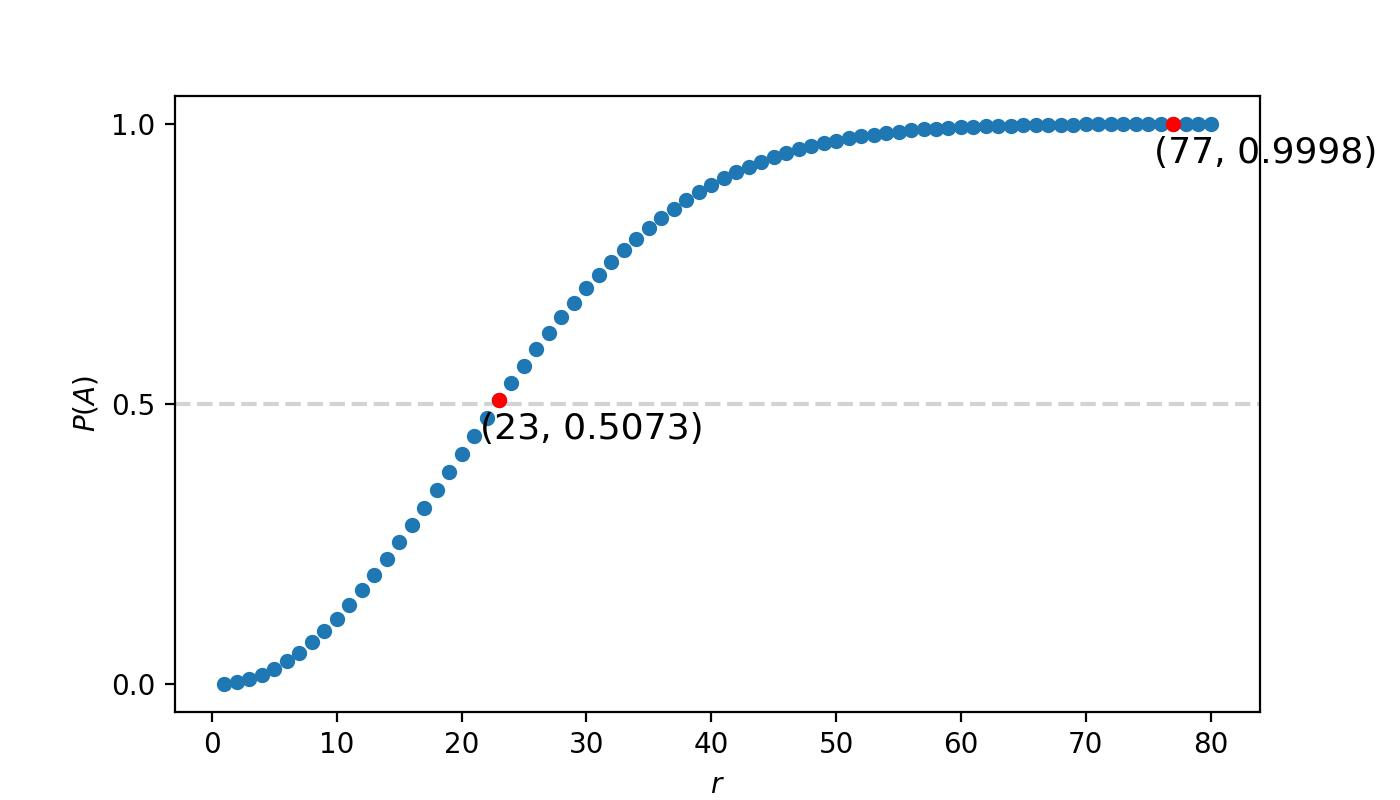
\includegraphics[scale = 0.7]{problema-cumple.jpg}
\end{figure}

\end{document}
